\begin{center}
{\LARGE ČESKÉ VYSOKÉ UČENÍ TECHNICKÉ V PRAZE\\}
	\vspace{10pt}
{\large FAKULTA JADERNÁ A FYZIKÁLNĚ INŽENÝRSKÁ\\}
{\large KATEDRA DOZIMETRIE A APLIKACE IONIZUJÍCÍHO ZÁŘENÍ\\}
	\vspace{40pt}
    
\includegraphics[width=0.25\textwidth]{cvut.jpg}
    %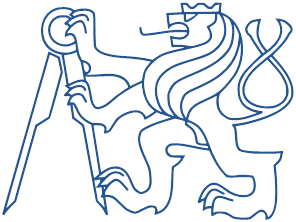
\includegraphics[scale=0.7]{cvut.png}

	\vspace{40pt}
{\Huge \textbf{BAKALÁŘSKÁ PRÁCE\\}}
	\vspace{10pt}
{\LARGE \textbf{Prostorová distribuce dávky uvnitř Mezinárodní kosmické stanice\\}}
	\vspace{150pt}

\end{center}
{\large
\begin{tabular}{p{4cm} p{8cm}}
Autor: & Michal Šesták\\
Vedoucí práce: & Ing. Iva Ambrožová, Ph.D.\\
Praha, 2017 & \\
\end{tabular}
}
%\newpage
%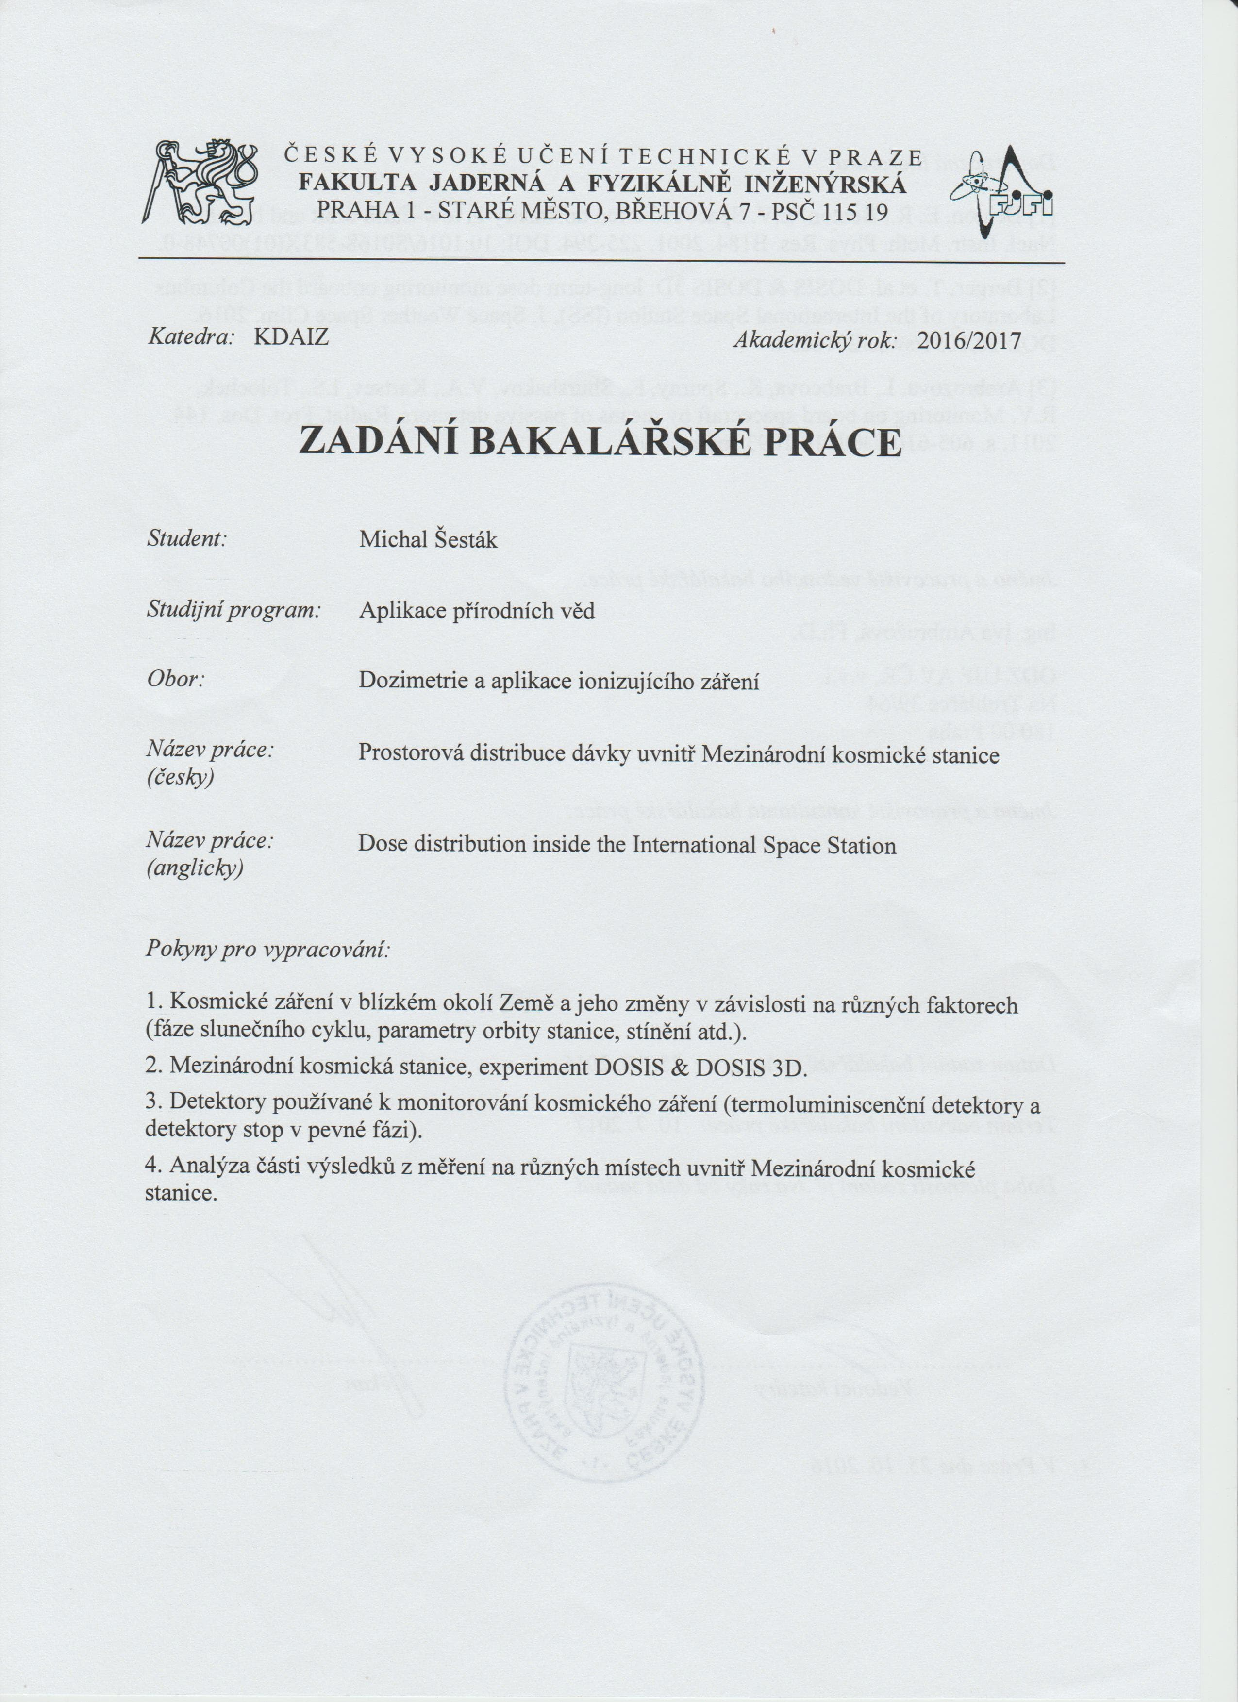
\includepdf[pages={1,2}]{parts/zadani.pdf}
\newpage
\vspace*{\fill}
\section*{Prohlášení}
Prohlašuji, že jsem svou bakalářskou práci vypracoval samostatně a použil jsem pouze podklady uvedené v přiloženém seznamu.\\[10pt]
V Praze dne \\[10pt]
\newpage
\vspace*{\fill}
\section*{Poděkování}
Děkuji Ing. Ivě Ambrožové, Ph.D. za vedení mé bakalářské práce, za cenné rady a připomínky, které tuto práci obohatily.
\newpage
\begin{tabularx}{\textwidth}{>{\itshape}l X}
  Název práce: & \textbf{Prostorová distribuce dávky uvnitř Mezinárodní kosmické stanice}\\
  Autor: & Michal Šesták\\
  Obor: & Dozimetrie a aplikace ionizujícího záření\\
  Druh práce: & Bakalářská práce\\
  Vedoucí práce: & Ing. Iva Ambrožová, Ph.D.\\ 
               & Oddělení dozimetrie záření, Ústav jaderné fyziky AV ČR, v.v.i., Akademie věd České republiky\\
  Abstrakt: & Kosmické záření představuje veliký zdravotní risk při pobytu ve vesmíru. K jeho monitorování se používají i pasivní detektory, obzvláště pak termoluminiscenční detektory a detektory stop v pevné fázi. Za účelem stanovení prostorové distribuce dávky uvnitř Mezinárodní kosmické stanice proběhlo a probíhá mnoho experimentů. Patří mezi ně i experimenty DOSIS (2009--2011) a DOSIS3D (2012--doposud). Z naměřených dat lze do určité míry vyvodit závislost dávkového příkonu na řadě parametrů, např. sluneční aktivitě a nadmořské výšce. 
  %Tato měření mohou zmenšit možné ozaření lidské posádky při budoucích letech do vesmíru.
  Tato práce pojednává o složení kosmického záření v blízkém okolí Země, o výše zmíněných pasivních detektorech, o projektech DOSIS a DOSIS3D a nakonec je uvedena názorná ukázka vyhodnocení tří detektorů stop, které byly umístěny v modulu Columbus. \\
  %Cílem práce bude studovat prostorovou distribuci dávkových veličin na různých místech ISS pomocí kombinace termoluminiscenčních detektorů a detektorů stop v pevné fázi, které byly poustupně umístěny na ISS v posledních několika letech. Student se seznámí s metodikou vyhodnocování detektorů, včetně měření a zpracování dat. \\
  Klíčová slova: & kosmické záření v blízkém okolí Země, detektory stop v pevné fázi, ISS, modul Columbus, DOSIS, DOSIS3D
\end{tabularx}
\newpage
\begin{tabularx}{\textwidth}{>{\itshape}l X}
  Title: & \textbf{Dose distribution inside the International Space Station}\\
  Author: & Michal Šesták\\
  Abstract: & Cosmic rays represents a huge health risk. Passive detectors are widely used for the measurement, especially thermoluminescent detectors and solid state nuclear track detectors. There were and are many experiments dealing with the determination of radiation environment within the International Space Station. Experiments DOSIS (2009--2011) and DOSIS3D (2012--so far) are two of them. The measured data can provide informations about influence of several parameters (for instance solar activity, altitude) to the dose rate. This thesis includes informations about characterictics of the cosmic rays in low Earth orbit, about passive detectors used in space measurements, about experiments DOSIS and DOSIS3D. There is also involved the evaluation of three track etched detectors at the end of the work.\\
  Key words: & cosmic rays in low Earth orbit, solid state nuclear track detectors, ISS, Columbus module, DOSIS, DOSIS3D
\end{tabularx}
\newpage 
%Experiment DOSIS was running between years 2009--2011 and its purpose was the determination of radiation environment within the International Space Station's Columbus module. Experiment DOSIS3D, which has started in 2012, has the same aim

